\section{The Gradient}
\noindent
If you are on a surface $f: \mathbb{R}^2 \to \mathbb{R}$, what direction $\langle \Delta x, \Delta y \rangle$ should you go to maximize the change of $f$?\\
We saw earlier that $\Delta z\approx \langle f_x, f_y \rangle \cdot \langle \Delta x, \Delta y \rangle$.
To maximize a dot product, $\langle \Delta x, \Delta y \rangle$ should be in the same direction as $\langle f_x, f_y \rangle$.
This directional vector is called the gradient: the direction of steepest ascent.\\
Notated mathematically,
\begin{equation*}
	\nabla f(x,y) = \langle f_x, f_y \rangle.
\end{equation*}

\begin{figure}[H]
	\centering
	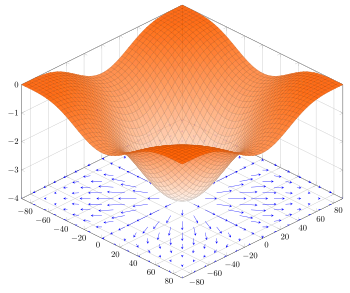
\includegraphics[width=0.5\textwidth]{./Images/differentialMultivariableCalculus/gradient.png}
	\caption{A surface and its gradient vectors}
\end{figure}

\subsection{Gradient Properties}
\noindent
Let $f$ and $g$ be functions of multiple variables, let $\vec{r}$ be a VVF, and let $c\in\mathbb{R}$.
\begin{enumerate}
	\item $\nabla(f\pm g)=\nabla f\pm\nabla g$
	\item $\nabla(cf)=c\nabla f$
	\item $\nabla(fg)=f\nabla g+g\nabla f$
	\item $\nabla(f\circ\vec{r}(t))=\nabla f\cdot\vec{r}(t)$
\end{enumerate}
\subsection{Linear Approximations with the Gradient}
\noindent
We can rewrite our linear approximation of $f$ at $x_0$ using the gradient.
\begin{equation*}
	f(x) \approx f(x_0) + (\nabla f)(x_0) \cdot (x - x_0)
\end{equation*}
\subsection{The Gradient \& C-Level Curves}
\noindent
Let $\vec{r}(t)$ be the C-level curve of $f(x, y)$.
\begin{align*}
f\circ\vec{r} &= C  \text{ and } \frac{\mathrm{d}}{\mathrm{d}t}(f\circ\vec{r}) = 0 \\
	&\implies \frac{\mathrm{d}}{\mathrm{d}t}(f\circ\vec{r}) = \nabla f\cdot\vec{r^\prime}(t) = 0 \\
	&\implies \nabla f\perp\vec{r^\prime}(t) \\
	&\implies \nabla f \text{ is perpendicular to the C-level curve of } f.
\end{align*}

[INSERT IMAGE]